\documentclass[9pt]{beamer}

\usetheme[progressbar=frametitle,block=fill,background=light]{metropolis}
\usefonttheme{serif}

\usepackage{appendixnumberbeamer}

\usepackage{booktabs}
\usepackage[scale=2]{ccicons}


\usepackage{pgfplots}
\usepgfplotslibrary{dateplot}
\usepackage{pgfplotsthemetol}
\usepackage{amsmath,amssymb,amsthm,amsfonts,amstext}
\usepackage{bbm}
\usepackage{array}
\usepackage{multimedia}
\usepackage{media9}
\usepackage{caption}
\usepackage{subcaption}

\usepackage{xspace}

\usepackage{import}
\import{}{Packages/custom_macros.tex}

\makeatletter
\setlength{\metropolis@titleseparator@linewidth}{2pt}
\setlength{\metropolis@progressonsectionpage@linewidth}{2pt}
\setlength{\metropolis@progressinheadfoot@linewidth}{2pt}
\makeatother

\newcommand{\themename}{\textbf{\textsc{metropolis}}\xspace}
\renewcommand{\emph}{\alert}
\newcommand{\pencil}{
\includegraphics[scale=0.07]{Pictures/pen.png}}
\renewcommand{\Re}{\text{Re}}
\renewcommand{\Im}{\text{Im}}

\title{Group theory, Topology and Spin-$1/2$ Particles}
\subtitle{From Dirac's belt to fermions}
% \date{\today}
\date{}
\author{Louan Mol}
\institute{Unversité Libre de Bruxelles\\[2cm]{\small Brussels Summer School of Mathematics 2022}}
% \titlegraphic{\hfill\includegraphics[height=1.5cm]{logo.pdf}}

\begin{document}

\maketitle

\nocite{*}

\begin{frame}{Table of contents}
    \setbeamertemplate{section in toc}[sections numbered]
    \tableofcontents%[hideallsubsections]
\end{frame}

\section{Dirac's belt trick and the rotation group}

\begin{frame}{Dirac's belt trick}
    
    You need:
    \begin{itemize}
        \item a belt (not necessarily Dirac's)
        \item a heavy book
    \end{itemize}

    \textbf{\underline{Goal:}}\\ [0.2cm]

    Deform the belt to untwist a $4\pi$-twist. Possible ? \visible<2->{\emph{Yes !}}\\[0.2cm]

    What about a $2\pi$-twist ? \visible<2->{\emph{No !} One turn negates the twist: $2\pi\to-2\pi$.}\\[0.2cm]

    \visible<2->{\textbf{\underline{Result:}} \\[0.2cm]
    
    The torsion in the belt rotates two times faster than the ends of the belt.\\[0.2cm]
    
    How can we explain that ?\\ [0.2cm]
    Very interesting mathematics are hiding behind this simple demonstration.}

\end{frame}

\begin{frame}{Mathematicalizing the belt}

    Mathematical description of the belt ?\\[0.3cm]
    \quad $\triangleright$ a belt is a strip, which is just a \emph{path} $+$ an \emph{orientation}.\\[0.2cm]
    \quad $\triangleright$ at each point along the middle the belt, we put a set of axis aligned \\ \hspace{0.5cm} with the belt. Each set of axis is a rotation of the initial set. \\[0.2cm]
    \quad $\triangleright$ this defines a continuous set of rotations or, more precisely, a \emph{path in \\ \hspace{0.5cm} $\SO(3)$}
    \begin{figure}
        \centering
        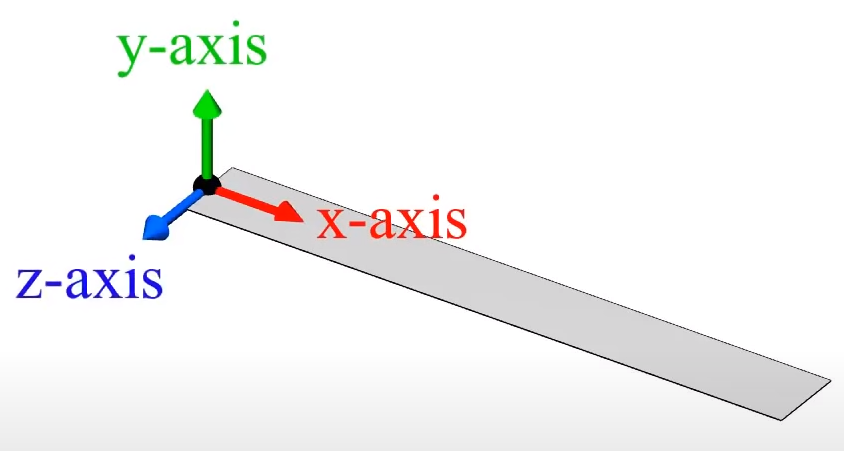
\includegraphics[scale=0.12]{Pictures/beltaxis.png}
    \end{figure}
    There is a bijection:
    \begin{equation*}
        \boxed{\text{belt configuration} \Leftrightarrow \text{path in $\SO(3)$}}
    \end{equation*}
    It provides us a new language to analyze the problem !

\end{frame}

\begin{frame}{Space of rotations}
      
    \textbf{\underline{As a matrix group:}}\\[0.2cm]

    A rotation is a real $3\times3$ matrix $R$ such that it
    \begin{enumerate}
        \item preserves the \emph{scalar product}: $R^TR=\mathbbm{1}$ ($\Leftrightarrow$ $R$ is orthogonal)
        \item preserves the \emph{orientation}: $\det R=1$
    \end{enumerate}

    \begin{block}{Special othogonal group}
        $\SO(3)$ is the set of $3\times 3$ real matrices such that $R^TR=\mathbbm{1}$ and $\det R=1$.
    \end{block}
    

    \visible<2->{
    \begin{columns}[T,onlytextwidth]
        \column{0.6\textwidth}

            \textbf{\underline{As a topological space:}}\\[0.2cm]

            Fundamentally, a rotation is a \emph{direction} + an \emph{angle}.\\
            $\Rightarrow$ it's a vector where the direction is the axis \\ \hspace{0.34cm} and the norm is the angle.\\[0.2cm]
            The set of all such vectors is
            \begin{equation*}
                \boxed{\SO(3)\cong B^3(\pi)/\sim}
            \end{equation*}
            Most famously known as $\R\P^3$.
  
        \column{0.4\textwidth}
  
            \begin{figure}
                \centering
                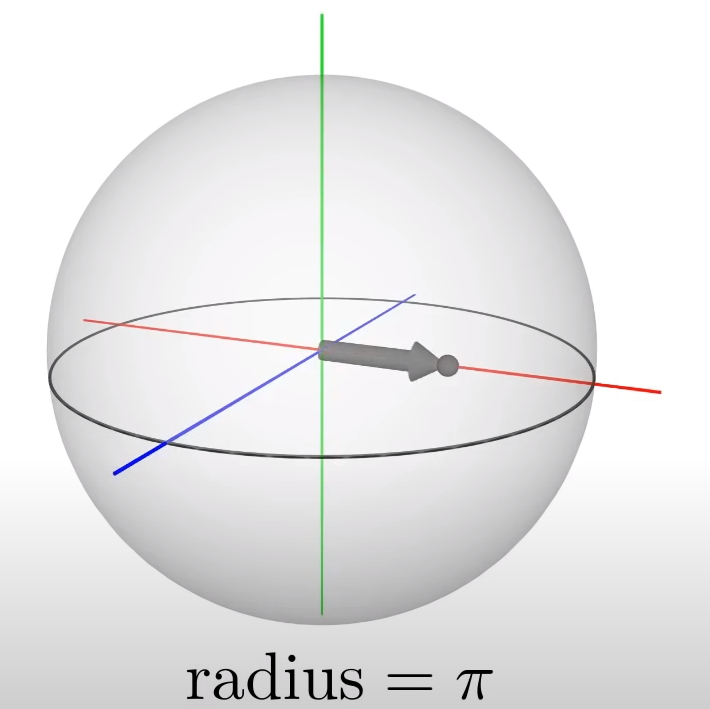
\includegraphics[scale=0.1]{Pictures/SO3sphere.png}
                \caption{$3$-sphere of radius $\pi$ with its antipodal points identified on the boundary.}
            \end{figure}
  
    \end{columns}}
    
\end{frame}



\begin{frame}{Examples}
    \makebox[315pt][r]{
    \begin{tabular}{cccc}
        \textbf{\underline{Trivial rotation}} & \textbf{\underline{$2\pi$ \textcolor{red}{$x$}-rotation}} & \textbf{\underline{$2\pi$ \textcolor{green}{$y$}-rotation}} & \textbf{\underline{$2\pi$ \textcolor{blue}{$z$}-rotation}}\\
        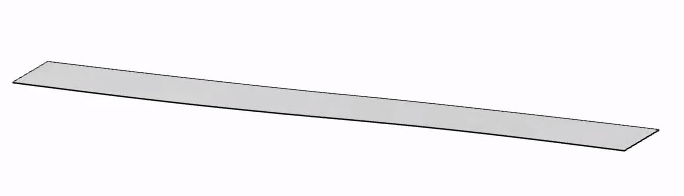
\includegraphics[scale=0.12]{Pictures/flatbelt.png} & 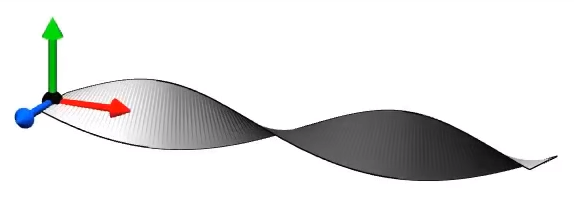
\includegraphics[scale=0.12]{Pictures/xaxisbelt.png} & 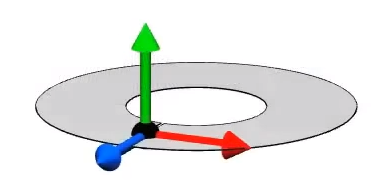
\includegraphics[scale=0.15]{Pictures/yaxisbelt.png} & 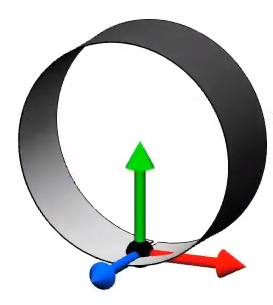
\includegraphics[scale=0.15]{Pictures/zaxisbelt.png} \\
        $\updownarrow$ & $\updownarrow$ & $\updownarrow$ & $\updownarrow$ \\
        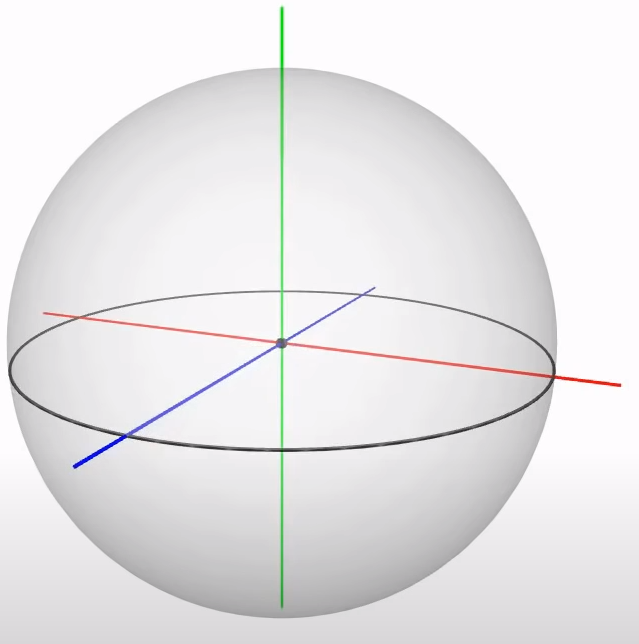
\includegraphics[scale=0.1]{Pictures/4pisphere4.png} & 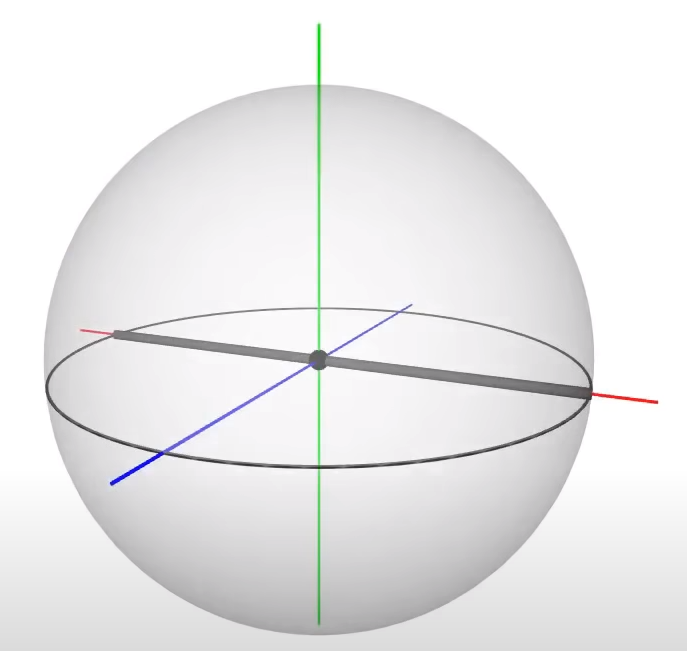
\includegraphics[scale=0.1]{Pictures/xaxissphere.png} & 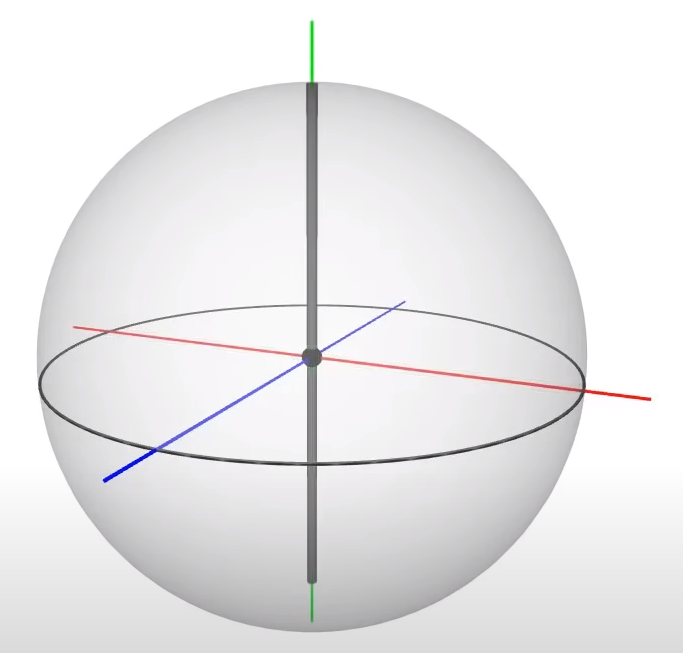
\includegraphics[scale=0.1]{Pictures/yaxissphere.png} & 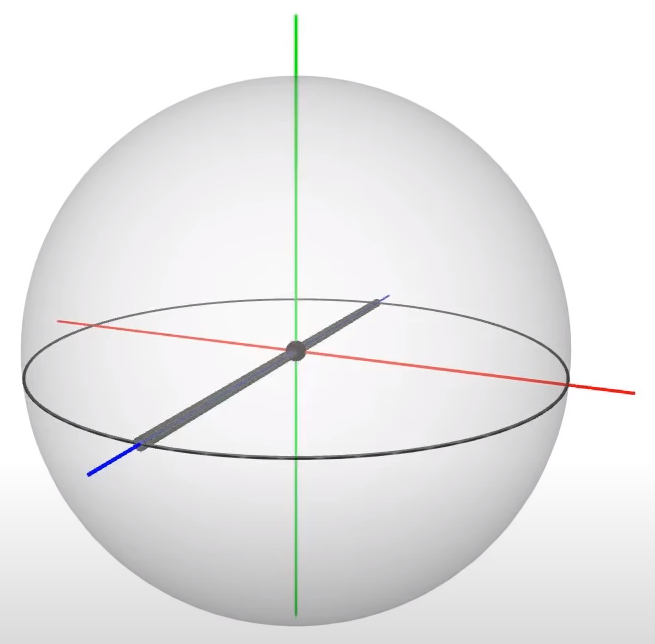
\includegraphics[scale=0.1]{Pictures/zaxissphere.png}
    \end{tabular}}
\end{frame}

\begin{frame}{Examples}
    \begin{center}
    \begin{tabular}{ccc}
        \textbf{\underline{Random path}} & \textbf{\underline{Closed path}} & \textbf{\underline{Open path}}\\
        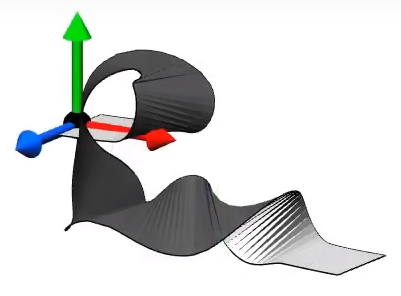
\includegraphics[scale=0.15]{Pictures/randomrotbelt.png} & 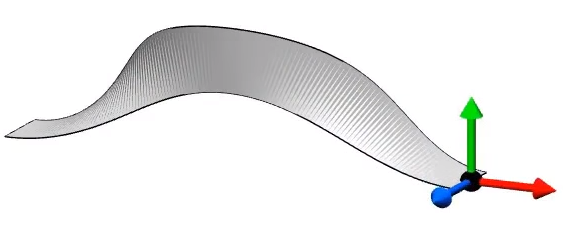
\includegraphics[scale=0.1]{Pictures/contractiblepathbelt.png} & 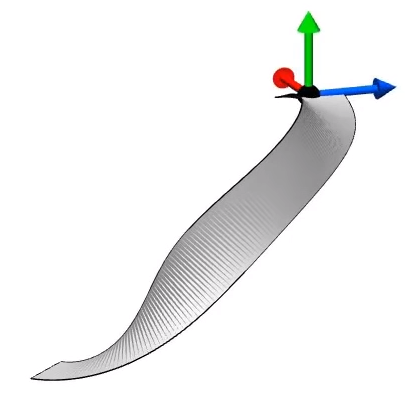
\includegraphics[scale=0.1]{Pictures/noncontractiblepathbelt.png} \\
        $\updownarrow$ & $\updownarrow$ & $\updownarrow$ \\
        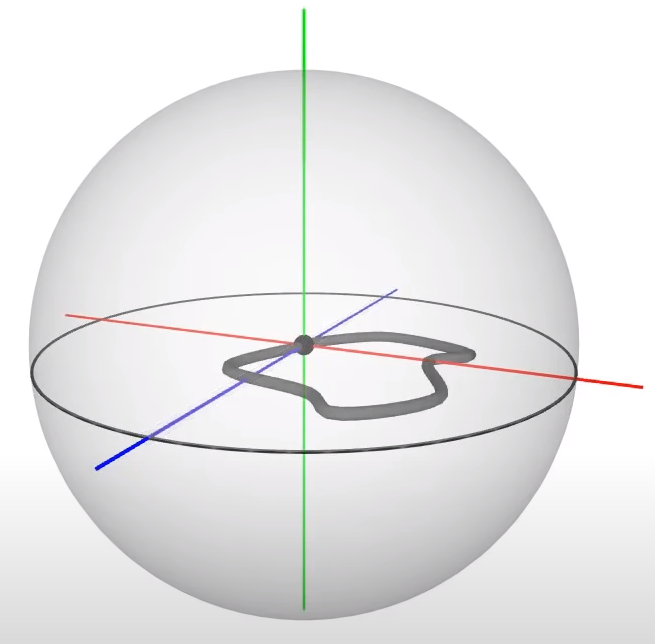
\includegraphics[scale=0.1]{Pictures/randomrotsphere.png} & 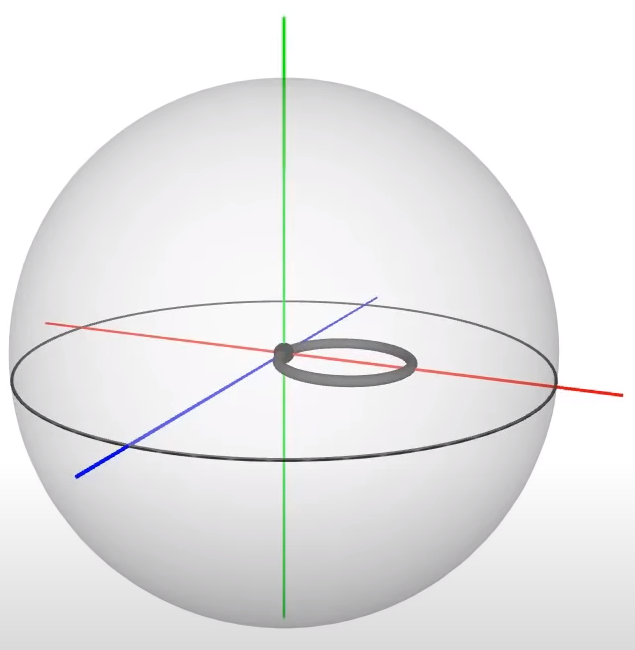
\includegraphics[scale=0.08]{Pictures/contractiblepathsphere.png} & 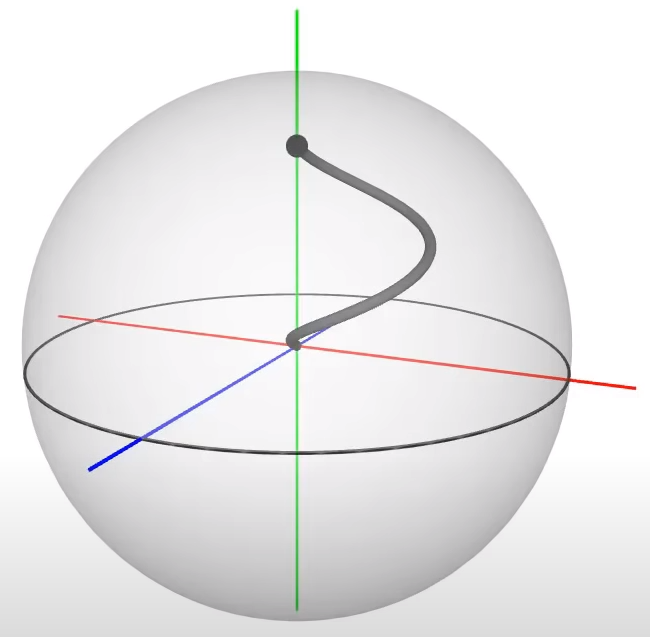
\includegraphics[scale=0.08]{Pictures/noncontractiblepathsphere.png}
    \end{tabular}
    \end{center}
\end{frame}

\begin{frame}{Dictionary}
    We see that:
    \begin{center}
    \begin{tabular}{|ccc|}
        \hline
        \textbf{\underline{Belt}} & & \textbf{\underline{Path}} \\[0.2cm]
        specific configuration & $\longleftrightarrow$ & specific path \\[0.2cm]
        moving the ends & $\longleftrightarrow$ & continuous deformation  \\[0.2cm]
        ends have same orientation & $\longleftrightarrow$ & loop \\[0.2cm]
        \emph{can be flattened} & $\longleftrightarrow$ & \emph{contractible} \\ \hline
    \end{tabular}
    \end{center}
    \textbf{Back to Dirac's belt trick:} the rules were
    \begin{enumerate}
        \item ends of the belt must keep the same orientation \textcolor{blue}{$\to$ we consider loops} \\
        \item moving the ends of the belt \textcolor{blue}{$\to$ continuous deformation} \\
        \item belt in original (flat) position \textcolor{blue}{$\to$ trivial constant path}
    \end{enumerate}
    The question ``can the belt be flattened ?'' then  ``\textbf{which loops are contractible ?}''
\end{frame}

\begin{frame}{Problem solved ?}
    \begin{itemize}
        \item \textbf{\underline{$4\pi$-twist:}}
    we saw in the beginning the the $4\pi$-twist can be flattened, how can we see this in terms of paths ?
    \begin{center}
        \begin{tabular}{m{2cm} m{0.5cm} m{2cm} m{0.5cm} m{2cm}}
            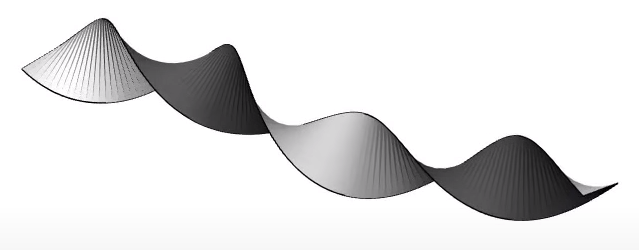
\includegraphics[scale=0.1]{Pictures/4pibelt.png} & $\longleftrightarrow$ & 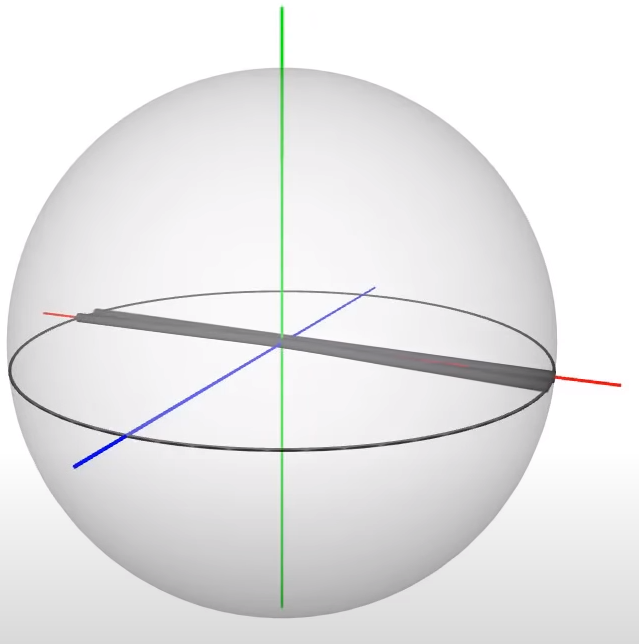
\includegraphics[scale=0.08]{Pictures/4pisphere1.png} & $\longrightarrow$ & 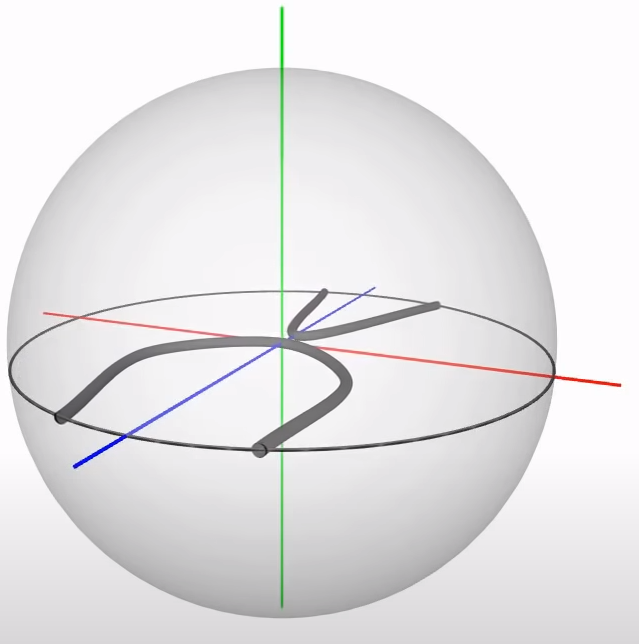
\includegraphics[scale=0.08]{Pictures/4pisphere2.png} \\
            & & & & \hspace{0.7cm} $\downarrow$ \\
            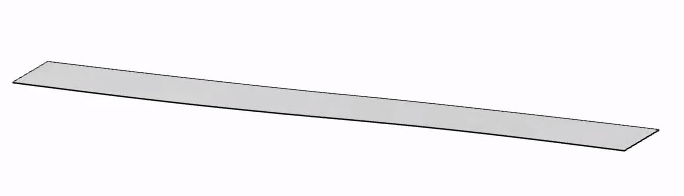
\includegraphics[scale=0.1]{Pictures/flatbelt.png} & $\longleftrightarrow$ & 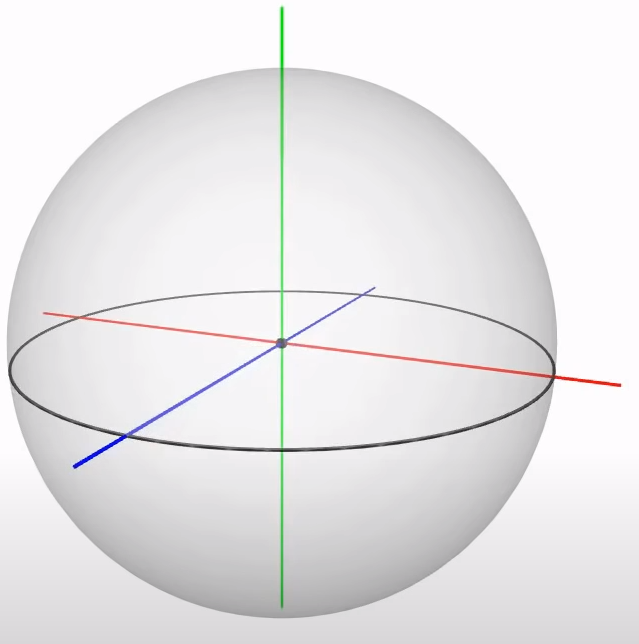
\includegraphics[scale=0.08]{Pictures/4pisphere4.png} & $\longleftarrow$ & 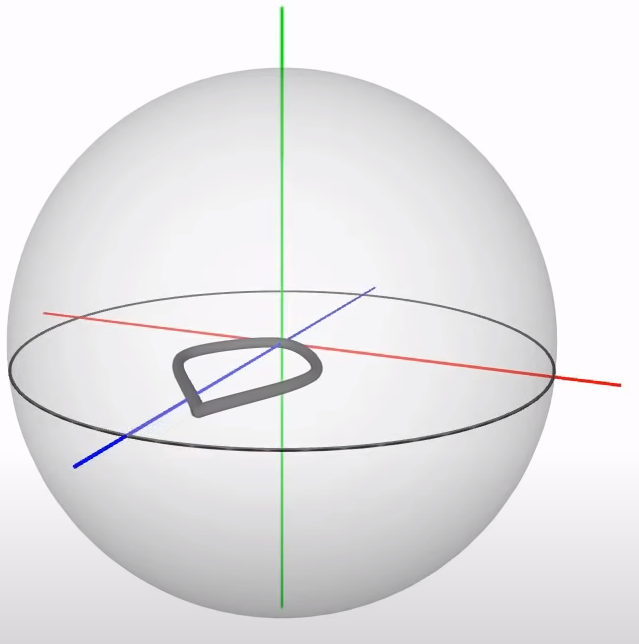
\includegraphics[scale=0.08]{Pictures/4pisphere3.png}
        \end{tabular}
    \end{center}
    $\Rightarrow$ the $4\pi$-twist is \emph{contractible} ! Great.
    \item \textbf{\underline{$2\pi$-twist:}} we ``clearly'' see that is not contractible... no ?! Great..?..  \\[0.2cm]
    \end{itemize}
    \textbf{Wierd aftertaste:} our ``proof'' is good to show contractibility but bad to show non-contractibility and it only works for simple examples.\\
    $\Rightarrow$ We want a consistent and general way of studying paths in topological spaces.
\end{frame}

\section{Homotopy theory}

\begin{frame}{Homotopoy theory primer}
    \textbf{Starting observation:} depending on the topological space, all loops might not be contractible. Moreover, some loops are ``fundamentally different'' from each other, e.g. in $\R^3$, $S^2$, $\mathbb{T}^2$, etc.

    \begin{block}{Paths and homotopies}
        For a topological space $X$:
        \begin{itemize}
            \item \textit{Path} in $X$: continuous map $\gamma:[0,1]\to X$,
            \item \textit{Loop} : closed path, i.e. embedded circle,
            \item $\gamma_1$ and $\gamma_2$ are \textit{homotopically equivalent} if one can be deformed into the other: there exists
            $f_t: [0,1]\to X$ with $t\in I$ such that
            \begin{equation*}
                f_0(s)=\gamma_1(s)\qquad \text{and}\qquad f_1(s)=\gamma_2(s).
            \end{equation*}
            and the endpoints are fixed. This is an equivalence relation ($\sim$).
        \end{itemize}
    \end{block}
    
    For each $x_0\in X$, we define
    \begin{equation*}
        \boxed{\pi_1(X,x_0) = \{\text{all loops based at }x_0\}/\sim,}
    \end{equation*}
    $\to$ set of ``fundamentally different'' loops passing through $x_0$.
\end{frame}

\begin{frame}{Fundamental group}
    The elements of $\pi_1(X,x_0)$ are $[\gamma]$, called the \textit{homotopy class} of $\gamma$.\\[0.2cm]
    Group structure on $\pi_1(X,x_0)$:
    \begin{itemize}
        \item \textbf{Product} of paths: $\gamma_1\cdot\gamma_2=$ ``$\gamma_1$ then $\gamma_2$''
        \item \textbf{Inverse} path: $\gamma^{-1}=$ ``$\gamma$ traversed in the opposite direction''
        \item \textbf{Neutral} path: $e=$ ``constant path at the identity''
        \item For homotopy classes: $[\gamma_1]\cdot[\gamma_2]=[\gamma_1\cdot\gamma_2]$ and $[\gamma]^{-1}=[\gamma^{-1}]$
    \end{itemize}
    Important fact: if $X$ is path-connected, $\pi_1(X,x_0)$ does not depend on $x_0$, up to isomorphism. \\ $\Rightarrow$ we denote it as $\pi_1(X)$, it is called the \emph{fundamental group} of $X$.\\[0.2cm]
    
    \visible<2->{Contractible loops are $\sim$ to a point, i.e. they are the elements of $[e]$.\\[0.2cm]

    \begin{block}{Proposition (product of spaces)}
        If $X$ and $Y$ are path-connected, $\pi_1(X\times Y)\cong\pi_1(X)\times\pi_1(Y)$.
    \end{block}
    \begin{block}{Proposition (maps between spaces)}
        If $\vp:X\to Y$ is a continuous map, it induces a homomorphism $\vp_*:\pi_1(X,x_0)\to\pi_1(Y,\vp(x_0))$ though $\vp_*([\gamma])=[\vp\circ\gamma]$.
    \end{block}}

\end{frame}

\begin{frame}{Computing the fundamental group}

    \textbf{How to compute $\pi_1(X)$ ?}\\[0.2cm]
    
    Can be difficult, there are different methods (e.g. Van Kampen theorem, Hopf fibrations, Hurewicz theorems, etc), not discussed here. A lot of homotopy groups are still unknown !\\[0.4cm]

    \begin{columns}[T,onlytextwidth]
        \column{0.55\textwidth}
        
            \textbf{Examples:}
            {\small
            \begin{enumerate}
                \item $\pi_1(\R^2)=0$
                \item $\pi_1(S^2) = 0$
                \item $\pi_1(S^1) = \Z$
                \item $\pi_1(\mathbb{T}^2)=\pi_1(S^1)\times\pi_1(S^1)=\textcolor{green}{\Z}\times\textcolor{red}{\Z}$
                \item $\pi_1(\R^2\backslash\{p\})=\Z$
            \end{enumerate}}
  
        \column{0.45\textwidth}
  
            \begin{figure}
                \centering
                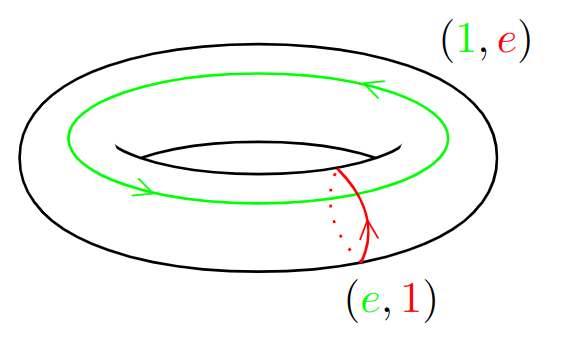
\includegraphics[scale=0.2]{Pictures/torushomotopy3.png}
            \end{figure}
  
    \end{columns}

    \visible<2->{\textbf{Remarks:} 
    \begin{itemize}
        \item $\pi_1(S^1)=\Z$ implies various famous theorems: fundamental theorem of algebra, Brouwer's fixed point theorem, Borusk-Ulam theorem etc.
        \item $\pi_1(\R^2\backslash\{p\})=\Z$ but $\pi_1(\R^3\backslash\{p\})=0$, higher homotopy groups for higher-dimensional holes ? Yes, \textit{$n$th homotopy group}:
        \begin{equation*}
            \pi_n(X,x_0)=\{\text{$S^n$ based at $x_0$}\}/\sim.
        \end{equation*}
    \end{itemize}}

\end{frame}

\begin{frame}{Homotopy groups of spheres}

    Good example of the complexity of homotpy groups:\\[0.2cm]
    \quad $\triangleright$ embedding a sphere in a higher-dimensional one: always trivial \\[0.2cm]
    \quad $\triangleright$ embedding a sphere in itself: always $\Z$ ways \\[0.2cm]
    \quad $\triangleright$ embedding a sphere in lower-dimensional one: much more complicated, \\ \hspace{0.5cm} periodic for a bit, then completely chaotic

    \visible<2->{
    \begin{figure}
        \centering
        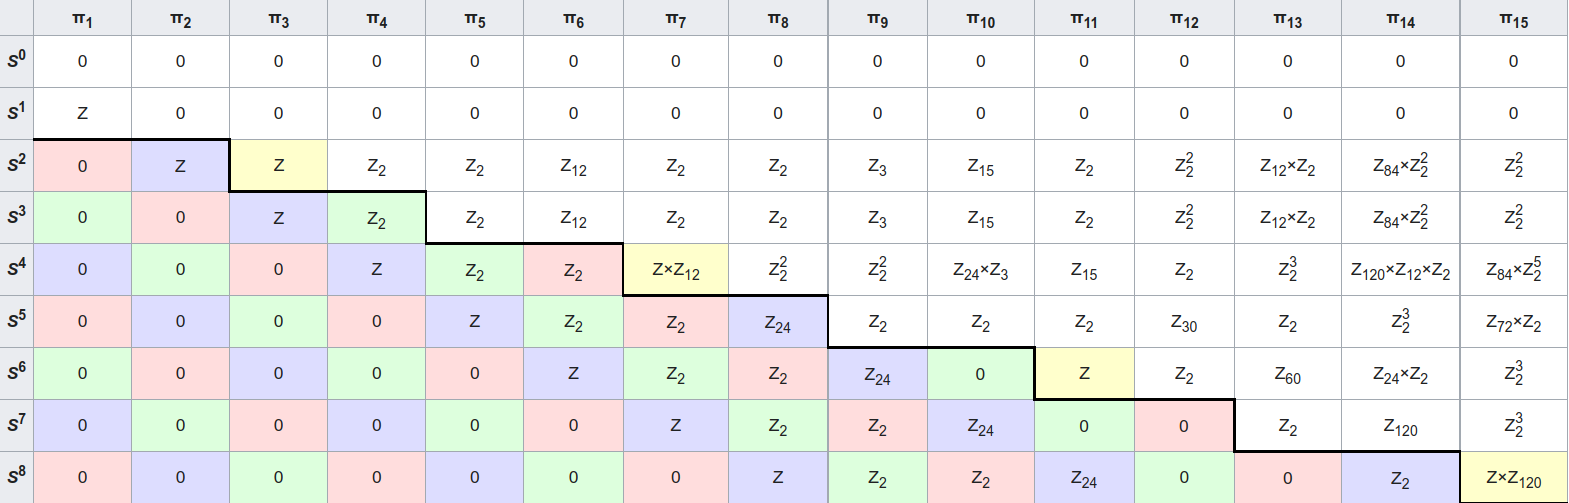
\includegraphics[scale=0.2]{Pictures/homotpoygroupsphere.png}
        \caption{Homotopy groups of spheres.}
    \end{figure}}


\end{frame}

\begin{frame}{Back to $\SO(3)$}
    \textbf{Question we had:} are all loops in $\SO(3)$ contractible ?\\
    In homotopy language: is $\pi_1(\SO(3))$ trivial ?\\[0.2cm]
    \visible<2->{
        \textbf{Answer:} \emph{NO}, one can show that
        \begin{equation*}
            \boxed{\pi_1(\SO(3))=\Z_2}
        \end{equation*}
        $\Rightarrow$ There only two ``fundamentally different'' loops in $\SO(3)$ !\\
        $\Rightarrow$ there is only one kind of non-contractible loop !\\[0.2cm]

        Indeed, there only two different initial configurations (i.e. two possible loops in $\SO(3)$):
        \begin{itemize}
            \item $4\pi k$-twists which are all equivalent
            \item $(4\pi k+2\pi)$-twists which are all equivalent
        \end{itemize}
        with $k\in\Z$.
    }\\[0.2cm]

    \visible<3->{
        We have a better understanding Dirac's belt trick. \textbf{But still no proof !} Homotopy theory allowed us to understand the ways of embedding loops in some spaces, we now need a tool to lift this ambiguity: \emph{covering spaces} !
    }

\end{frame}

\section{Covering spaces}

\begin{frame}{Covering spaces}
    
    \begin{columns}[T,onlytextwidth]
        \column{0.75\textwidth}
        
            \begin{block}{Covering space}
                For a topological space $X$, a \textit{covering space} is a topological space $\tilde{X}$ with a \textit{projection map} $p:\tilde{X}\to X$ such that there exists an open cover $\{\U_\alpha\}$ for which $p^{-1}(U_\alpha)$ is a disjoint union of open sets in $\tilde{X}$, each of which is mapped by $p$ homeomorphically on $U_\alpha$. \\
                If $X$ is connected, $|p^{-1}(x)|$ is constant and called the number of \textit{sheets}.
            \end{block}

            \textbf{\underline{Examples}}\\
            There are many possibilities to cover the circle:
            \begin{itemize}
                \item $\R$ covers $S^1$ with $p_1(t)=(\cos(2\pi t),\sin(2\pi t))$,
                \item $\R$ covers $S^1$ with $p_2(t)=(\cos(5 t),\sin(5 t))$,
                \item $S^1$ covers $S^1$ in several ways, with $p(z)=z^n$, $n\in\N$.
            \end{itemize}
  
        \column{0.25\textwidth}
  
            \begin{figure}
                \centering
                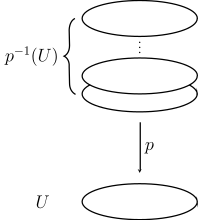
\includegraphics[scale=0.35]{Pictures/Covering_space_diagram.png}
            \end{figure}

            \begin{figure}
                \centering
                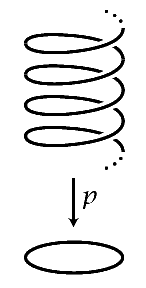
\includegraphics[scale=0.35]{Pictures/UniversalCoveringOfCircle.png}
            \end{figure}
  
    \end{columns}
    
\end{frame}

\begin{frame}{General properties}

    \begin{itemize}
        \visible<1->{
        \item \textbf{Some covering spaces are equivalent:}
            \begin{minipage}{10cm}
                \begin{block}{Isomorphisms}
                    Two covering space $\tilde{X}$ and $\tilde{X}'$ of $X$ are \textit{isomorphic} if there exists a homeomorphism $h:\tilde{X}\to \tilde{X}'$ such that $p_2\circ h=p_1$.
                \end{block}
            \end{minipage}
            \textcolor{blue}{For $S^1$, $p_1$ and $p_2$ are isomorphic.}}\\[0.1cm]
        \item \visible<2->{\textbf{The lifting of point can, by definition, be ambiguous:}
            \begin{minipage}{10cm}
                \begin{block}{Deck transformations}
                    A \textit{Deck transformation} is a homeomorphism $d:\tilde{X}\to \tilde{X}$ such that $p\circ d=p$. With composition, they form a group $G(\tilde{X})$.
                \end{block}
            \end{minipage}
            \textcolor{blue}{For $S^1$, $G(\R)=\Z$ and $G(S^1)=\Z_n$.}}\\[0.1cm]
        \item \visible<3->{\textbf{Many covering spaces for the same base space:}
            \begin{minipage}{10cm}
            \begin{block}{Universal covering space}
                If $\tilde{X}$ is simply connected and $X$ is (locally) path-connected, there exists covering space of any other covering space. It is maximal, unique and called \textit{universal covering space} (UCS).
            \end{block}
            \end{minipage}
            \textcolor{blue}{$\R$ is the UCS of $S^1$.}}
    \end{itemize}

\end{frame}

\begin{frame}{Lifting properties}

    \begin{columns}[T,onlytextwidth]
        \column{0.8\textwidth}

        Observation:

        \begin{enumerate}
            \item Lifting points is ambiguous.
            \item Lifting path is not ambiguous if the starting point is fixed.
            \item Constant paths are lifted to constant paths.
            \item The projection of a homotopy is a homotopy for the projected paths.
            \item The lifts of homotopy-equivalent paths are homotopically equivalent! \textcolor{blue}{$\to$ relation between $\pi_1(X)$ and $\tilde{X}$ ?}
        \end{enumerate}

        \visible<2->{If $\tilde{X}$ is the UCS of $X$, we actually have
        \begin{equation*}
            \boxed{\pi_1(X)=G(\tilde{X}).}
        \end{equation*}
        }

        \column{0.2\textwidth}
  
        \begin{figure}
            \centering
            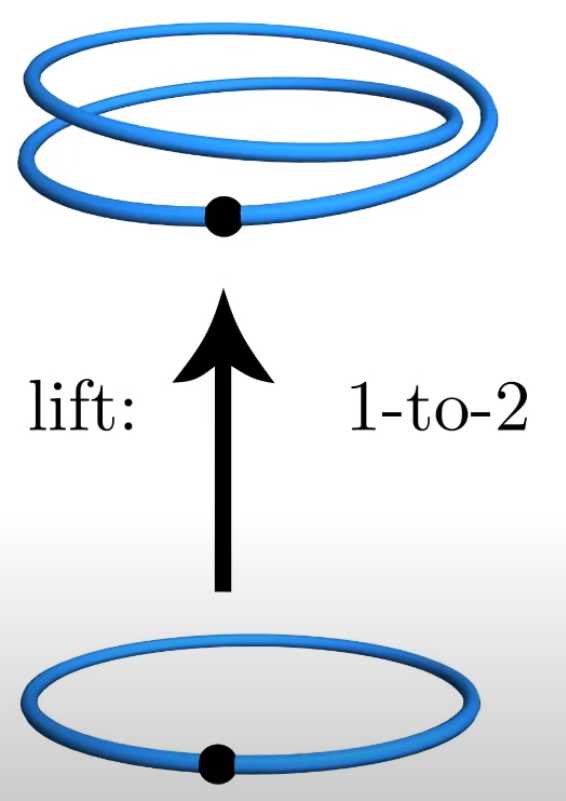
\includegraphics[scale=0.1]{Pictures/lifting_point.png}
        \end{figure}
        \begin{figure}
            \centering
            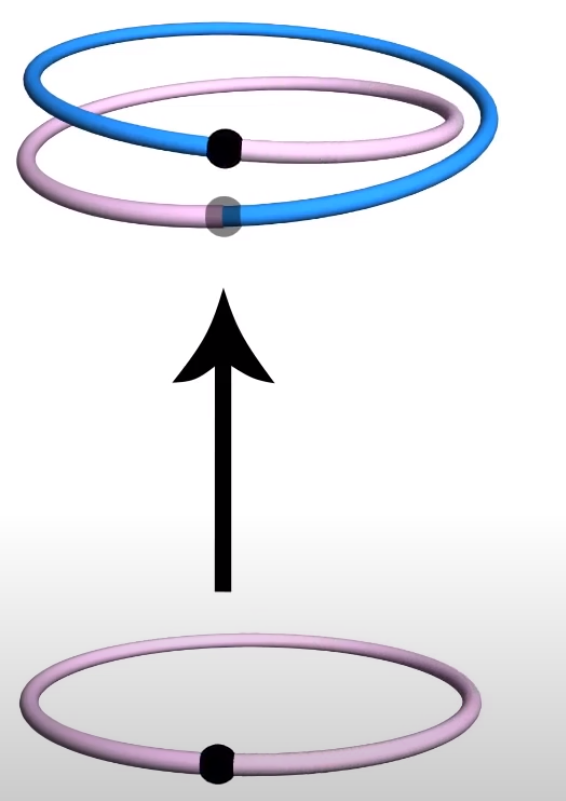
\includegraphics[scale=0.1]{Pictures/lifting_path.png}
        \end{figure}
  
    \end{columns}

        \visible<2->{$\Rightarrow$ algebraic features of $\pi_1(X)$ can be seen as geometric features of $\tilde{X}$.}

\end{frame}

\begin{frame}{Covering space of $\SO(3)$}

    One can show that
    \begin{equation*}
        \boxed{\text{The universal covering space of $\SO(3)$ is $\SU(2)$}.}
    \end{equation*}

    \begin{block}{Special unitary group}
        $\SU(2)$ is the set of $2\times 2$ complex matrices such that $U^\dagger U=\mathbbm{1}$ and $\det U=1$.
    \end{block}
    \visible<2->{\textbf{\underline{Properties of $\SU(2)$:}}\\
    What is the most general element of $\SU(2)$ ? Imposing $U^\dagger=U^{-1}$ and $\det U=1$, we find
    \begin{equation}
        U=
        \begin{bmatrix}
            X+iY & Z+iW \\
            -Z+iY & X-iY
        \end{bmatrix}
    \end{equation}
    with $X^2+Y^2+Z^2+W^2=1$ $\Rightarrow \SU(2)\cong S^3$.}\\[0.1cm]
    \visible<3->{\textbf{\underline{$\SU(2)$ and $\SO(3)$:}}
    \begin{enumerate}
        \item both of dimension three
        \item both are connected
        \item both isometry groups
        \item $-\mathbbm{1}\in\SU(2)$ but $-\mathbbm{1}\notin\SO(3)$
    \end{enumerate}}
\end{frame}

\begin{frame}{Representating $\SU(2)$}

    \begin{columns}[T,onlytextwidth]
        \column{0.65\textwidth}
        
        How could we represent $\SU(2)\cong S^3$ in $3d$ ?\\[0.2cm]

        Observation: $S^2$ is equivalent to two disks glued along their boundary.\\[0.2cm]

        Similarly, $S^3$ is equivalent to balls glued along their boundary.\\[0.2cm]

        \textbf{Question:} are those balls related to $\SO(3)$ ?\\[0.2cm]

        \visible<2->{They are the \emph{sheets} !}
            
        \column{0.35\textwidth}
  
            \begin{figure}
                \centering
                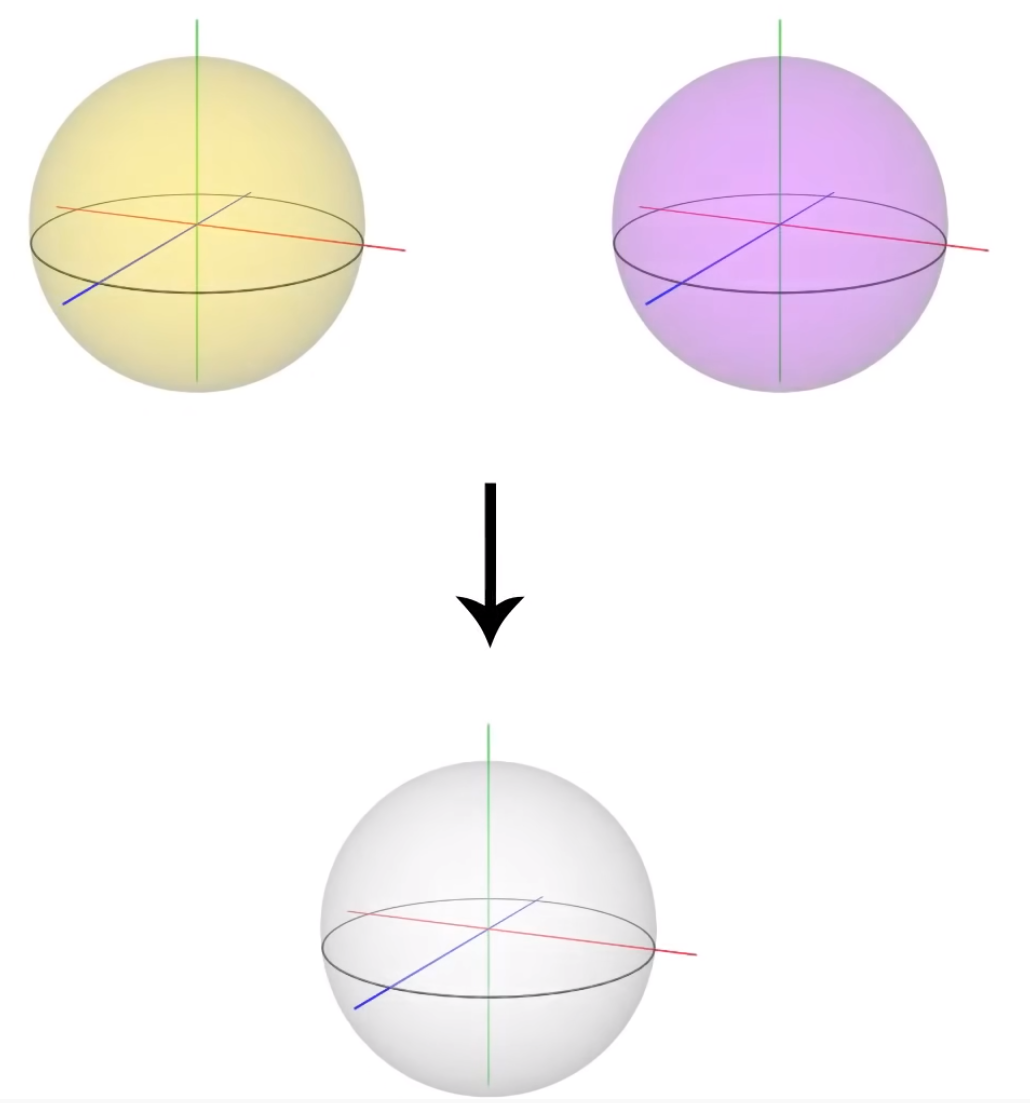
\includegraphics[scale=0.1]{Pictures/lifting_su2.png}
            \end{figure}
  
    \end{columns}

    \visible<2->{The projection map is
    \begin{equation*}
        p\left(\begin{bmatrix}
            x & y \\
            -\bar{y} & \bar{x}
        \end{bmatrix}\right)=
        \begin{bmatrix}
            \Re(x^2-y^2) & \Im(x^2+y^2) & -2\Re(xy) \\
            -\Im(x^2-y^2) & \Re(x^2+y^2) & 2\Im(xy) \\
            2\Re(x\bar{y}) & 2\Im(x\bar{y}) & \abs{x}^2-\abs{y}^2
        \end{bmatrix}
    \end{equation*}
    with $\abs{x}^2+\abs{y}^2=1$.}
    
\end{frame}


\begin{frame}{$\SU(2)$ and $\SO(3)$}

    \textbf{\underline{Group relation:}}\\[0.2cm]
    The fact that $\SU(2)$ is a \emph{double}-cover of $\SO(3)$ can can see in practice with
    \begin{equation*}
        p(U)=p(-U).
    \end{equation*}
    Intuitively, we should be able to recover $\SO(3)$ from $\SU(2)$ if $U\sim-U$. And, indeed,
    \begin{equation*}
        \boxed{\SO(3)\cong\SU(2)/\Z_2,}
    \end{equation*}
    where the quotient means exactly that we identity $U$ with $-U$.\\[0.2cm]

    \visible<2->{\textbf{\underline{Other formulation:}}\\[0.2cm]

    We saw that $S^3$ is a universal double-sheeted cover of $\R\P^3$, $\pi_1(S^3)=\{e\}$, and $\pi_1(\R\P^3)=\Z_2$. This makes sense since 
    \begin{equation*}
        \R\P^3=S^3/\{(x,y,z)\sim(-x,-y,-z)\}=S^3/\Z_2=\SU(2)/\Z_2,
    \end{equation*}
    we get the previous group relation.}

\end{frame}

\begin{frame}{Bringing it all together}

    What are the lifts of the $2\pi$-twist and the $4\pi$-twist ?
    \begin{align*}
        \text{$2\pi$-twist} &\to \text{path from $I$ to $-I$}\\
        \text{$4\pi$-twist} &\to \text{path from $I$ to $-I$ to $I$ again}
    \end{align*}
    \visible<2->{\textbf{\underline{Proof that $2\pi$-twist is non-contractible in $\SO(3)$:}}
    \begin{flushright}
    \begin{minipage}{10.5cm}
        Let us suppose that the $2\pi$-twist is contractible. At each step of its contraction, we can lift the path to $\SU(2)$. This provides us with a contraction of the lifted $2\pi$-twist. However, the lifted $2\pi$-twist does not have the same start and endpoint, therefore it is not contractible, and so is the non-lifted path.
    \end{minipage}
    \end{flushright}}
    \visible<3->{\textbf{\underline{Proof that $4\pi$-twist is contractible in $\SO(3)$:}}
    \begin{flushright}
    \begin{minipage}{10.5cm}
        The lift of the $4\pi$-twist is a loop. Since $\pi_1(\SU(2))=\pi_1(S^3)=0$, this loop is necessarily contractible. Projecting each step of its contraction provides us with a contraction of the $4\pi$-twist path in $\SO(3)$.
    \end{minipage}
    \end{flushright}}

\end{frame}

\begin{frame}{Summary of the analysis of Dirac's belt trick}

    \begin{itemize}
        \item Belt configurations are equivalent to paths in $\SO(3)$. New question: we want to classify the contractable and non-contractable loops.
        \item Fundamental groups and covering spaces: $\pi_1(X)$ and $\tilde{X}$ are two pictures of the same thing. $\tilde{X}$ is the space that contains the same information plus the topological information of non-equivalent paths, i.e. it ``solves'' the homotopy ambiguity.
        \item The UCS of $\SO(3)$ is $\SU(2)$, and it is a double cover.
        \item There only two kinds topologically-distinguishable loops: $[4\pi k\text{-twists}]$ is contractible and the $[(4\pi k+2\pi)\text{-twists}]$ is not contractible.
    \end{itemize}

    \begin{center}
        \begin{tabular}{|l|}
            \hline
            The belt trick is a way of physically demonstrating that the \\ fundamental group of $\SO(3)$ is $\Z_2$.\\ \hline
        \end{tabular}
    \end{center}
    
    \visible<2->{\textbf{Are there other manifestations of homotopy in our practical world ?}\\[0.2cm]

    Yes: the \emph{spin} ! (You don't need a belt, but you need an electron.)\\[0.1cm]
    Initially, this trick was a demonstration invented by Paul Dirac (1902-1984) to explain the notion of spin to his students.}

\end{frame}


\section{Quantum spin}

\begin{frame}{What is the spin ?}

    Skipping most of the physics background:
    \begin{block}{Spin in quantum mechanics}
        \begin{enumerate}
            \item The \textit{spin}  is an inherent property of any ``particle'':
            \begin{itemize}
                \item it's a number $s\in\frac{1}{2}\N$\textcolor{blue}{, in our case $s=1/2$}
                \item does not change (like the mass, charge, etc)
                \item classifies particles
            \end{itemize}
            \item A particle of spin $s$ is, at a given moment, in a certain state described by the \textit{spin vector}:
            \begin{itemize}
                \item unit vector of $v\in\C^{2s+1}$\textcolor{blue}{, in our case $\begin{bmatrix}\alpha\\ \beta\end{bmatrix}\in\C^2$}
                \item this state can evolve over time
            \end{itemize}
            \item What we can measure yet another quantity, called \textit{observed spin}:
            \begin{itemize}
              \item discrete value $s_{\text{obs.}}\in\{s,s-1,\dots,0,\dots,-s+1,-s\}$\\
              \textcolor{blue}{in our case, $s_{\text{obs.}}\in\{1/2,-1/2\}$ that we denote $\uparrow$ and $\downarrow$}
              \item given a direction, e.g. $i=x,y,z$
              \item outcome is random, QM predicts the probability of each outcome
            \end{itemize}
        \end{enumerate}
    \end{block}

\end{frame}

\begin{frame}{What is the spin ?}
    \textbf{How do measures happen ?}\\[0.2cm]
    Let us introduce
    {\tiny
    \begin{align*}
        v_{x,\uparrow}=
        \begin{bmatrix}
            1/\sqrt{2} \\ 1/\sqrt{2}
        \end{bmatrix},
        v_{x,\downarrow }=
        \begin{bmatrix}
            1/\sqrt{2} \\ -1/\sqrt{2}
        \end{bmatrix},
        v_{y,\uparrow}=
        \begin{bmatrix}
            1/\sqrt{2} \\ i/\sqrt{2}
        \end{bmatrix},
        v_{y,\downarrow}=
        \begin{bmatrix}
            1/\sqrt{2} \\ -i/\sqrt{2}
        \end{bmatrix},
        v_{z,\uparrow}=
        \begin{bmatrix}
            1 \\ 0
        \end{bmatrix},
        v_{z,\downarrow}=
        \begin{bmatrix}
            0 \\ 1
        \end{bmatrix}.
    \end{align*}}
    The probability of measuring $s_{\text{obs.}}$ in the direction $i$ is given by the projection
    \begin{equation}
        P(i,s_{\text{obs.}}) = \abs{\langle v_{i,s_{\text{obs.}}},v \rangle_{\C^2}}^2
    \end{equation}
    where $v$ is the spin vector of the particle and $\langle v,w \rangle=v^\dagger w$ is a scalar product on $\C^2$.\\[0.2cm]
    \textbf{Example}: in the direction $z$,
    \begin{equation}
      P(z,\uparrow)= \abs{\alpha}^2,\qquad P(z,\downarrow)= \abs{\beta}^2.
    \end{equation}
    Consequently:
    \begin{itemize}
        \item we must have $\langle v,v\rangle_{\C^2}=\abs{\alpha}^2+\abs{\beta}^2=1$
        \item to ``measure'' the spin state, we must repeat the experience many times
        \item there are states that are always spin $\uparrow$ or always spin $\downarrow$
    \end{itemize}
\end{frame}

\begin{frame}{The bizarre nature of fermions}

    \textbf{\underline{How to rotate a spin vector ?}}\\[0.2cm]
    We need to leave the probabilities conserved $\Rightarrow$ scalar product invariant:
    \begin{equation*}
        \boxed{\text{Spin vectors transform under $\SU(2)$ !}}
    \end{equation*}

    \visible<2->{\textbf{\underline{How do space rotations act on spin vectors ?}}\\[0.2cm]
    The rotation group of euclidean space is still $\SO(3)$, so we need a way of doing an $\SO(3)$ rotation through $\SU(2)$ transformations.\\[0.2cm]

    This is exactly what the covering technology provides us: a unique way to lift a rotation from $\SO(3)$ to $\SU(2)$.}\\[0.2cm]

    \visible<3->{\textbf{\underline{Interpretation ?}}\\[0.2cm]

    The $2\pi$-twist is not closed $\Rightarrow$ \emph{walking around} such a particle would not give back the particle in the same states, it would \emph{negate the spin state}. Very odd property ... Could such exotic particles exist ? Error of interpretation ?\\[0.2cm]}
    \visible<4->{\emph{Yes}, they do exist! Out of the $18$ elementary particles, $12$ of them have spin $1/2$ ! And this have been observed experimentally.}

\end{frame}

\begin{frame}{The bizarre nature of fermions}

    \begin{figure}
        \centering
        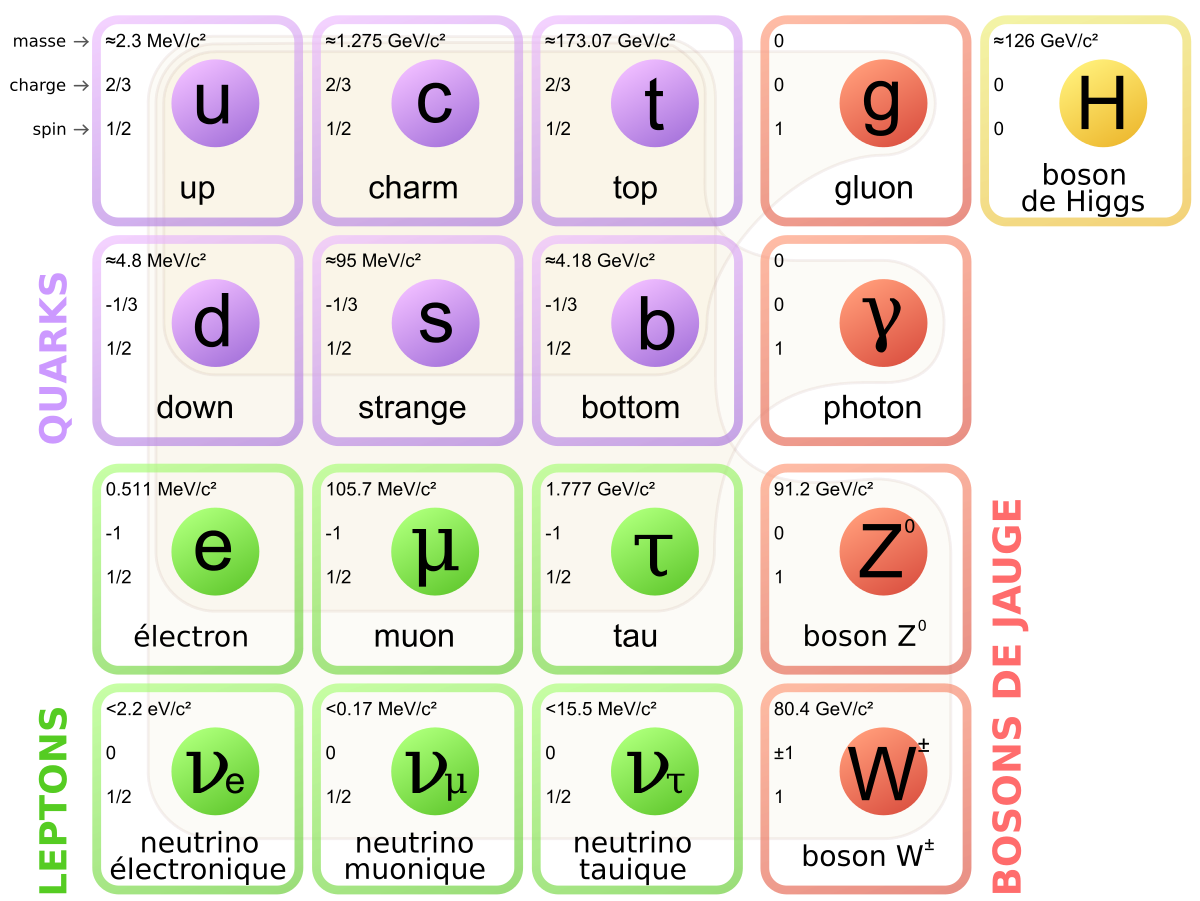
\includegraphics[scale=0.14]{Pictures/SM.png}
        \caption{Standard Model of particle physics.}
    \end{figure}

    {\small\textbf{\underline{Practical details:}}
    \begin{itemize}
        \item Instead of walking around the particle, we rotate it using a magnetic field (Lamor procession).
        \item We cannot detect the ```$-$'' sign if only one particle, at least two are necessary.
        \item We do not actually use electrons but neutrons (see neutron interferometry).
    \end{itemize}}
    
\end{frame}

\begin{frame}{Generalizations}

    \textbf{Other spins:} $s\in\frac{1}{2}\N$.\\[0.1cm]
    \textbf{Other dimensions:} $\SO(3)\to\SO(n)$ and $\SU(2)\to\Spin(n)$.\\[0.1cm]
    \begin{block}{Spinor}
        A \emph{spinor} of spin $s$ in dimension $n$ is an a element of $\C^{2s+1}$ transforming under a (complex) linear representation of $\Spin(n)$.
    \end{block}

    \visible<2->{\textbf{\underline{Summary on spinors:}}

    \begin{enumerate}
        \item There are two topologically distinguishable classes of paths through rotations that result in the same overall rotation. (True in any dimension, $\Spin(n)$ is always double-sheeted.) 
        \item The most general object should take that difference into account: spinors.
        \item A spinor is characterized by its \emph{spin}. Depending on the dimension of the space, the dimensions of the spin representations vary but all spins are always possible.
        \item Other approach: Clifford algebra !
    \end{enumerate}}

    % we discussed something for in three dimensions (with SO(3) and SU(2)), how can we generalize this ?
    % motivation: any rotation in R^3 can be achived in two topologically inequivalent ways, why should objects be blind to that ? The most general object is spinors
    % how to distinguish the topologically inequivalent rotations ? Universal cover of the group, double cover, spin groups
    % properties of the spin groups; in any dimension, actully always TWO topologically inequivalent ways of achieving a rotation, i.e. it is always a DOUBLE cover, it is unique, maximal, etc
    % def of spinor
    % other definition of spinor: Clifford algebras, def the algebra
    % link with the other definition: Both the spin group and its Lie algebra are embedded inside the Clifford algebra in a natural way, and in applications the Clifford algebra is often the easiest to work with.
    % representation theory of the CLifford algebra, i.e. spinors in all dimensions
    % come back the three dimensions, our example of SU(2) etc, with representations theory of SO(3) and SU(3), integer spin and half-interger spins

    % there are essentially two frameworks for viewing the notion of a spinor.

    % ccl the integer spin particles are vector repr (called bosons), they don't care about the homotopy class, the half integer spins are proper spinors, they caeer about the homotopy class, they are sensible to an additional Z_2 (called fermions).


\end{frame}

\begin{frame}{Ending remarks on spinors}

    \textbf{\underline{Spin in nature:}}
    \begin{itemize}
        \item only spins $0$ (Higgs boson), $1/2$ (electrons, quarks, etc), $1$ (photons, gluons, etc) and $2$ (graviton) are found in nature
        \item spins higher than $2$ are technically very problematic, and not well-understood yet. Current topic of research (U Mons !)
        \item spin-$1/3$ particles ? No, impossible, because $\pi_1(SO(3))=\Z_{\textcolor{red}{2}}$. Example of mathematical constraint on physical models.
    \end{itemize}
    %modern fundamental physics is relativistic so we use a pseudo-scalar product. The isometry group becomes $\SO(1,3)$. The spinor theory we depicted can be generalized to $\SO(p,q)$.

    \visible<2->{\textbf{\underline{Behind quantum mechanics:}} \\[0.2cm]

    The spinors we encountered previously are spinors in Quantum Mechanics, which is non-relativistic. Modern Physics is relativistic therefore we mainly care about the \emph{indefinite rotation groups} rather than the usual rotation groups, because of \emph{special relativity}. The whole theory can be generalized accordingly:

    \begin{figure}
        \centering
        \begin{tabular}{c|cc}
            & \textbf{Non-relativistic} & \textbf{Relativistic} \\ \hline
            rotation group & $\SO(3)$ & $\SO(1,3)$ \\
            UCS & $\Spin(3)=\SU(2)$ & $\Spin(1,3)=\SL(2,\C)$
        \end{tabular}
    \end{figure}}

\end{frame}

\section{More belts, more fun}

{
\setbeamercolor{background canvas}{bg=black!100}
\begin{frame}{Anti-twister mechanisms}
    \begin{center}
        \movie[width=10cm,height=5.5cm,showcontrols,loop]{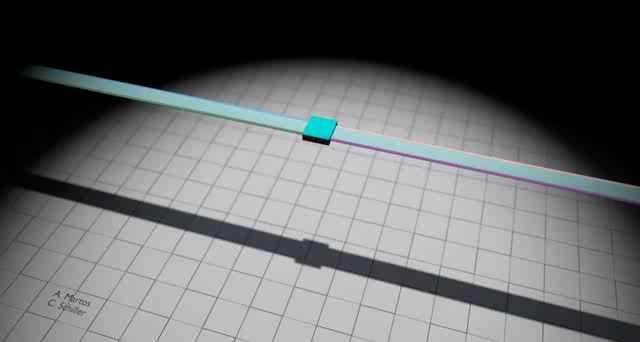
\includegraphics[scale=0.25]{Pictures/poster2belts.jpg}}{Videos/2belts.wmv}
    \end{center}
    {\small\textcolor{white}{Expanding the Dirac's belt trick setup, one can attach two belts to an object and rotate it by 720° without it getting tangled. Combining the two movements, the object can spin continuously without becoming tangled.}}
\end{frame}}

{
\setbeamercolor{background canvas}{bg=black!100}
\begin{frame}{Anti-twister mechanisms}
    \begin{center}
        \movie[width=10cm,height=5.5cm,showcontrols,loop]{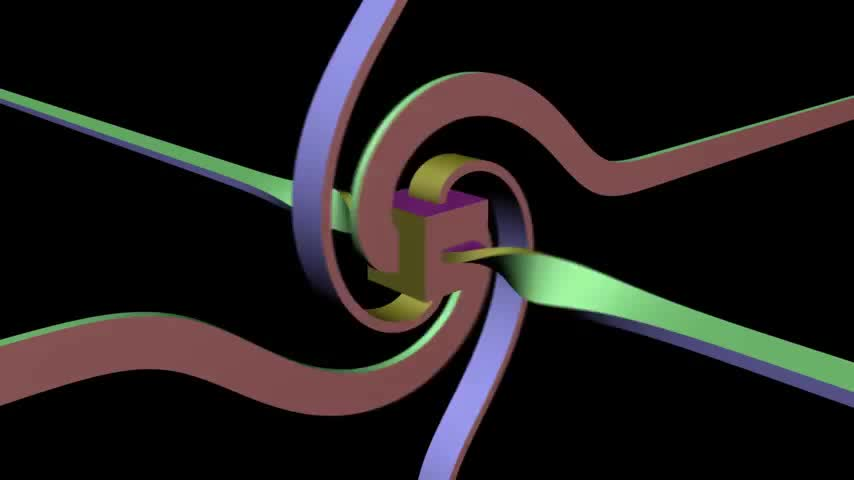
\includegraphics[scale=0.25]{Pictures/poster1.jpg}}{Videos/video1.wmv}
    \end{center}
    {\small\textcolor{white}{Increasing the number of belts does not change this behavior. Notice that after the cube completed a 360° rotation, the spiral is reversed from its initial configuration. It only returns to its original configuration after spinning a full 720°.}}
\end{frame}}

{
\setbeamercolor{background canvas}{bg=black!100}
\begin{frame}{Anti-twister mechanisms}
    \begin{center}
        \movie[width=10cm,height=5.5cm,showcontrols,loop]{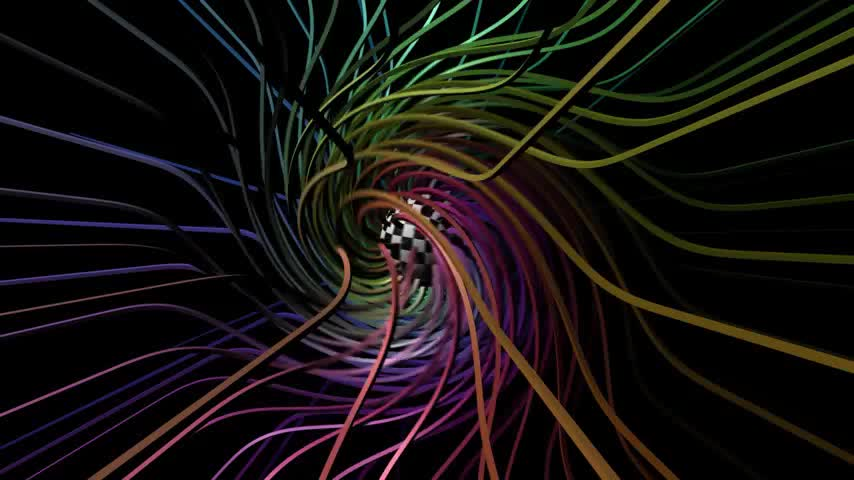
\includegraphics[scale=0.25]{Pictures/poster2.jpg}}{Videos/video2.wmv}
    \end{center}
    {\small\textcolor{white}{A more extreme example demonstrating that this works with any number of strings. In the limit, a piece of solid continuous space can rotate in place like this without tearing or intersecting itself.}}
\end{frame}
}

% https://bloerg.net/posts/beamer-movies-and-linux/

\begin{frame}{Fun facts}

    \begin{itemize}
        \item Anti-twister mechanisms are used in engineering to supply electric power to rotating devices.
        \item The cup on the hand trick (balinese candle dance or Philippine wine dance).
        \item Tangloids is mathematical gamed base on the same principles.
        \item Link with quaternions.
    \end{itemize}

    \begin{figure}
        \centering
        \begin{subfigure}[b]{0.5\textwidth}
            \centering
            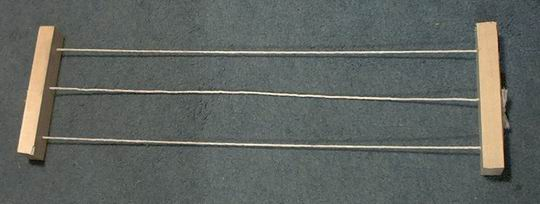
\includegraphics[scale=0.2]{Pictures/Tangloids.jpeg}
            \caption{Tangloids.}
        \end{subfigure}\begin{subfigure}[b]{0.5\textwidth}
            \centering
            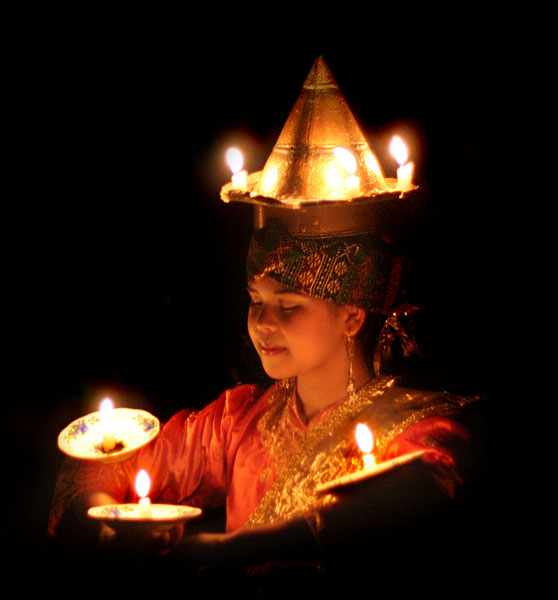
\includegraphics[scale=0.2]{Pictures/balinesedance.jpg}
            \caption{Balinese candle dance.}
        \end{subfigure}
   \end{figure}

\end{frame}

% tangloids
% videos on 
% anti-twister mechanism: The anti-twister or antitwister mechanism is a method of connecting a flexible link between two objects, one of which is rotating with respect to the other, in a way that prevents the link from becoming twisted. The link could be an electrical cable or a flexible conduit. This mechanism is intended as an alternative to the usual method of supplying electric power to a rotating device. What makes the device possible is the peculiar connectivity of the space of 3D rotations, as discovered[3] by P. A. M. Dirac and illustrated in his Plate trick (also known as the string trick or belt trick).[4] Its covering Spin(3) group can be represented by unit quaternions, also known as versors.

\section{Conclusion}

\begin{frame}{Conclusion}

    \begin{enumerate}
        \item Dirac's belt trick can be understood by studying the fundamental group of $\SO(3)$.
        \item The universal cover of $\SO(3)$ is $\SU(2)$, in which the homotopy ambiguity is solved. Spin vectors transform under $\SU(2)$ and covering space technology then allows us to better understand the nature of the spin in quantum mechanics.
        \item Spinors can be defined in any dimension and for any spin. Leading to a generalization of usual vectors that take into account the topological difference between some rotations that, a priori, could look equivalent.
        \item Spinors are fundamental in modern theories of fundamental interactions. Spinors model most of elementary particles. In particular, exactly like Dirac's belt, electrons rotate through the lift in $\SU(2)$ thus taking into account the homotopy class of the rotation, how cool ?!
    \end{enumerate}
    \vspace{0.5cm}
    \visible<2->{
    \begin{center}
        {\huge\textit{Thank you !}}
    \end{center}}

\end{frame}

\appendix

\begin{frame}{More on rotations}

    Three ``fundamental'' rotations:
    \begin{equation*}
      {\tiny
      x:
      \begin{bmatrix}
          1 & 0 & 0 \\
          0 & \cos\theta & -\sin\theta \\
          0 & \sin\theta & \cos\theta
      \end{bmatrix}\qquad
      y:
      \begin{bmatrix}
          \cos\theta & 0 & -\sin\theta \\
          0 & 1 & 0 \\
          \sin\theta & 0 & \cos\theta
      \end{bmatrix}\qquad
      z:
      \begin{bmatrix}
          \cos\theta & -\sin\theta & 0 \\
          \sin\theta & \cos\theta & 0 \\
          0 & 0 & 1
      \end{bmatrix}}
    \end{equation*}
    any rotation can be obtained by composing those three rotation.\\[0.2cm]
    Bijection between rotations and unit quaternions:
    \begin{equation*}
        (\overrightarrow{n},\theta)\qquad\Leftrightarrow\qquad e^{\frac{\theta}{2}(n_x\textbf{i}+n_y\textbf{j}+n_z\textbf{k})}=\cos\frac{\theta}{2}+(n_x\textbf{i}+n_y\textbf{j}+n_z\textbf{k})\sin\frac{\theta}{2}
    \end{equation*}
    using an extension of Euler's formula. Then,
    \begin{itemize}
        \item rotation of a vector $\overrightarrow{r}$: $\textbf{p}'\to \textbf{q}\textbf{p}\textbf{q}^{-1}$ with $\textbf{p}=r_x\textbf{i}+r_y\textbf{j}+r_z\textbf{k}$,
        \item composition of rotations: $\textbf{q}=\textbf{q}_1\textbf{q}_2$.
    \end{itemize}
    
\end{frame}


\begin{frame}{Construction of the projection map}
    
    We introduce the \textit{Pauli matrices}(generators of $\mathfrak{su}(2)$):
    \begin{equation}
        \sigma_1 =
        \begin{bmatrix}
            0 & 1\\
            1 & 0
        \end{bmatrix},\qquad
        \sigma_2 =
        \begin{bmatrix}
            0 & -i\\
            i & 0
        \end{bmatrix},\qquad
        \sigma_3 =
        \begin{bmatrix}
            1 & 0\\
            0 & -1
        \end{bmatrix}.
    \end{equation}
    Then, for $\overrightarrow{r}=(x,y,z)\in\R^3$, the matrix
    \begin{equation*}
        \overrightarrow{r}\cdot \overrightarrow{\sigma}=r^i\sigma_i=
        \begin{bmatrix}
            z & x-iy\\
            x+iy & -z
        \end{bmatrix}
    \end{equation*}
    is \emph{traceless} and \emph{self-adjoint}, i.e. $\overrightarrow{r}\cdot \overrightarrow{\sigma}\in\mathfrak{su}(2)$. More precisely, $\sigma_i$ are the generators of $\mathfrak{su}(2)$. Moreover $\det(\overrightarrow{r}\cdot \overrightarrow{\sigma})=-(x^2+y^2+z^2)$.\\[0.2cm]
    We can then shown that, the new matrix $U(\overrightarrow{r}\cdot \overrightarrow{\sigma})U^\dagger$, with $U\in\SU(2)$ is 
    \begin{itemize}
        \item still traceless and self-adjoint \\
            $\Rightarrow$ $\exists \overrightarrow{r}_U\in\SO(3)$ such that $U(\overrightarrow{r}\cdot \overrightarrow{\sigma})U^\dagger=\overrightarrow{r}_U\cdot \overrightarrow{\sigma}$
        \item has same determinant, i.e $\abs{\overrightarrow{r}}=\abs{\overrightarrow{r}_U}$\\
            $\Rightarrow$ $\exists R_U\in\SO(3)$ such that $\overrightarrow{r}_U=R\overrightarrow{r}$
    \end{itemize}
    In then end, for each $U\in\SU(2)$, we have $p(U)\equiv R_U\in\SO(3)$. This maps can be shown to be locally a \emph{homeomorphism}.
\end{frame}

\begin{frame}{More on homotpy}

    \begin{block}{Proposition}
        If $\vp:X\to Y$ are is a homotopy equivalence, then the induced homomorphism $\vp_*:\pi_1(X,x_0)\to\pi_1(Y,\vp(x_0))$ is an isomorphism for all $x_0\in X$.
    \end{block}
    \begin{block}{Theorem (fundamental theorem of algebra)}
        Every non-constant polynomial with coefficients in $\C$ has a root in $\C$.
    \end{block}
    \begin{block}{Theorem (Brouwer fixed point)}
        Every continuous map $h:D^2\to D^2$ has a fixed point.
    \end{block}
    \begin{block}{Theorem (Borusk-Ulam)}
        For every continuous map $f=S^2\to \R^2$ there exist a pair of antipodal points $x$ and $-x$ in $S^2$ such that $f(x)=f(-x)$.
    \end{block}

    One can generalize and show that $\pi_n(S^n)=\Z$. These theorems are then generalized accordingly.
    
\end{frame}

\begin{frame}{More belts}
    We can see that
\end{frame}

\begin{frame}{References}

    \bibliography{bibliography}
    \bibliographystyle{abbrv}

\end{frame}

\end{document}
